% exercise sheet with header on every page for math or close subjects
\documentclass[12pt]{article}
\usepackage[utf8]{inputenc} 
\usepackage{latexsym} 
\usepackage{multicol}
\usepackage{fancyhdr}
\usepackage{amsfonts} 
\usepackage{amsmath}
\usepackage{amssymb}
\usepackage{enumerate}
\usepackage{listings}
\usepackage{graphicx}
\usepackage{float}


% Shortcuts for bb, frak and cal letters
\newcommand{\E}{\mathbb{E}}
\newcommand{\V}{\mathbb{V}}
\renewcommand{\P}{\mathbb{P}}
\newcommand{\N}{\mathbb{N}}
\newcommand{\R}{\mathbb{R}}
\newcommand{\C}{\mathbb{C}}
\newcommand{\Z}{\mathbb{Z}}
\newcommand{\Pfrak}{\mathfrak{P}}
\newcommand{\Pfrac}{\mathfrak{P}}
\newcommand{\Bfrac}{\mathfrak{P}}
\newcommand{\Bfrak}{\mathfrak{B}}
\newcommand{\Fcal}{\mathcal{F}}
\newcommand{\Ycal}{\mathcal{Y}}
\newcommand{\Bcal}{\mathcal{B}}
\newcommand{\Acal}{\mathcal{A}}


% Formatierung
\topmargin -2cm 
\textheight 24cm
\textwidth 16.0 cm 
\oddsidemargin -0.1cm

\setlength{\parindent}{0pt}  % !!!!!!! Hier werden leerzeilen erlaubt ohne dass Latex automatisch einrueckt! !!!!!!! %


\graphicspath{ {images/} }


\begin{document}

% Titel
%\title{\textsc{Hacking}\\ \textsc{Abgabe 0}\\{ \normalsize Gruppe X \hfill Daniel Schäfer (2549458)\\ \hfill Anderer}}
%\maketitle  

% alternativer Titel
\noindent
{\Large \textbf{High-level Computer Vision}} \hfill \textbf{22.06.2016}\\
{\Large \textbf{Exercise 5}} 
\raggedleft \hfill Guillermo Reyes (2556018)\\
\hfill Daniel Schaefer (2549458)\\
\hfill Marc Tonsen (2537359)\\
\hfill Dominik Weber (2548553)\\

\pagenumbering{gobble}
\raggedright



\section{Data Augmentation}

\begin{enumerate}[a)]
        \setcounter{enumi}{1}
    \item 
        %TODO
        % flip occurs in batch and thus the flipped pictures are different after every get_batch, results in overall 'more' training data
        \begin{figure}[H]
            \centering
                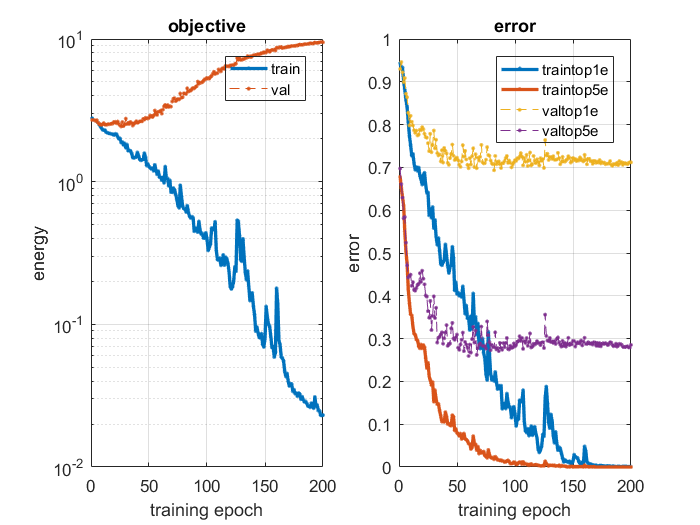
\includegraphics[width=0.9\textwidth]{Plots/init_plot_epo_200.png}
                \caption{without using left-right mirroring}
        \end{figure}
        \begin{figure}[H]
            \centering
                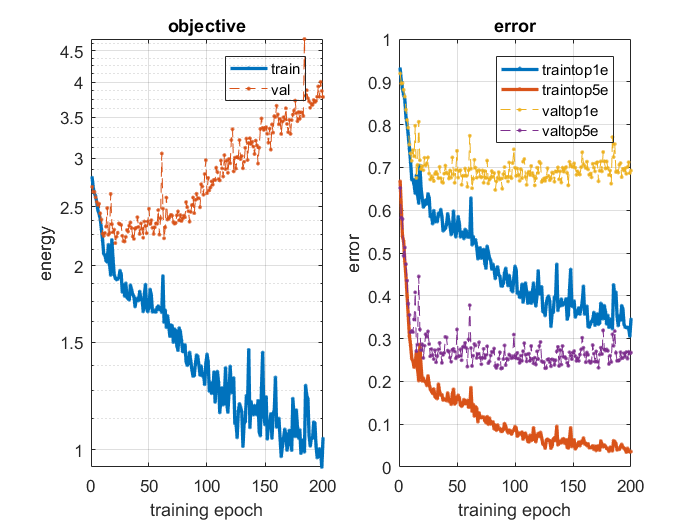
\includegraphics[width=0.9\textwidth]{Plots/q1_plot_epo_200.png}
                \caption{with using left-right mirroring}
        \end{figure}
        Using jittering as we do effectively doubles the amount of images the network gets to see. As long as left-right mirroring the data does not create images that are highly unrealistic (which is not the case for us), this is reasonable to do. This results in less overfitting (the gap between train and test error remains smaller) and the best test error is smaller: 0.65 vs 0.70 without jittering.
		Also the training-error decreases more slowly, which is understandable, since the data presented to the network in each epoch changes a lot due to the jittering, which makes it more difficult for the network to adept to it correctly.

\end{enumerate}


\newpage
\section{Mean Image Substraction}

\begin{enumerate}[a)]
        \setcounter{enumi}{1}
    \item 
        We should not use both sets at once to compute the mean, because in that case the test data would have an impact on our training which would compromise the evaluation. Instead only the image-mean of the training data should be substracted from both the training data and the test data. The test-data should not be transformed differently than the training-data because the distribution of the test data must not be altered differently than the distribution of the training data to ensure the equality of both  distributions. 
    \item
        The best validation error decreased from 0.72 to 0.64 in our Plot.
        \begin{figure}[H]
            \centering
                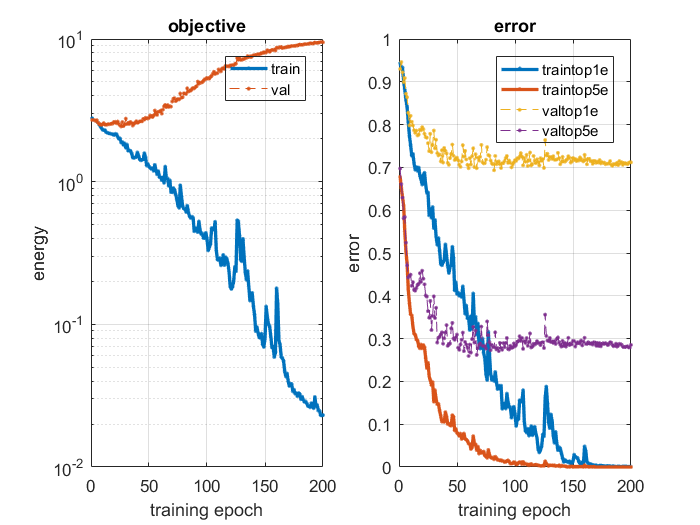
\includegraphics[width=0.9\textwidth]{Plots/init_plot_epo_200.png}
                \caption{without using mean-image substraction}
        \end{figure}
        \begin{figure}[H]
            \centering
                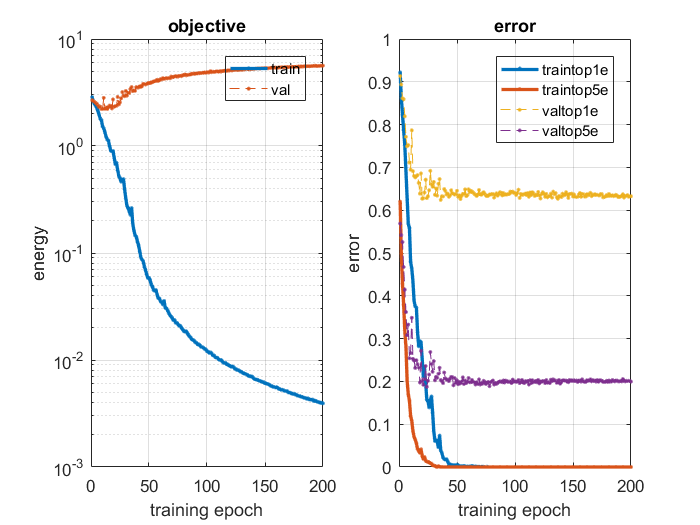
\includegraphics[width=0.9\textwidth]{Plots/q2_plot_epo_200.png}
                \caption{with using mean-image substraction}
        \end{figure}
        Also the validation error seems to decrease faster.\\
        Similar to the case using not mean subtraction the training error quickly decreases further while the validation error remains roughly on the same level, which indicates overfitting.
\end{enumerate}


\newpage
\section{Dropout}

\begin{enumerate}[a)]
    \item 
        The idea of dropout is very similar to the one behind random forests. Random forests are an ensemble of decision trees. Each single decision tree is very prone to overfitting to the training-data. The random forest simply picks the average result out of all decision trees, which effectively cancels out the overfitting to a high amount. Dropout intuitively does the same: it trains several subsets of the network on the training-data and ''takes the average'' of them. This prevents the network from overfitting to the training data.
    \item
        Of cause not! At test-time we want to utilize the full power of the network. Discarding a part of it would discard the predictive power of that part as well, which in turn weakens the prediction made by the network.
    \item
        %TODO nicht eindeutig eins besser, haengt von daten ab. Dann noch spezifisch schreiben wie es bei uns aussieht und was wie gut wird/ist
        Using our Implementation a dropout of 50\% resulted in the lowest error (testing 200epochs) with around 0.66 error 
        \begin{figure}[H]
            \centering
                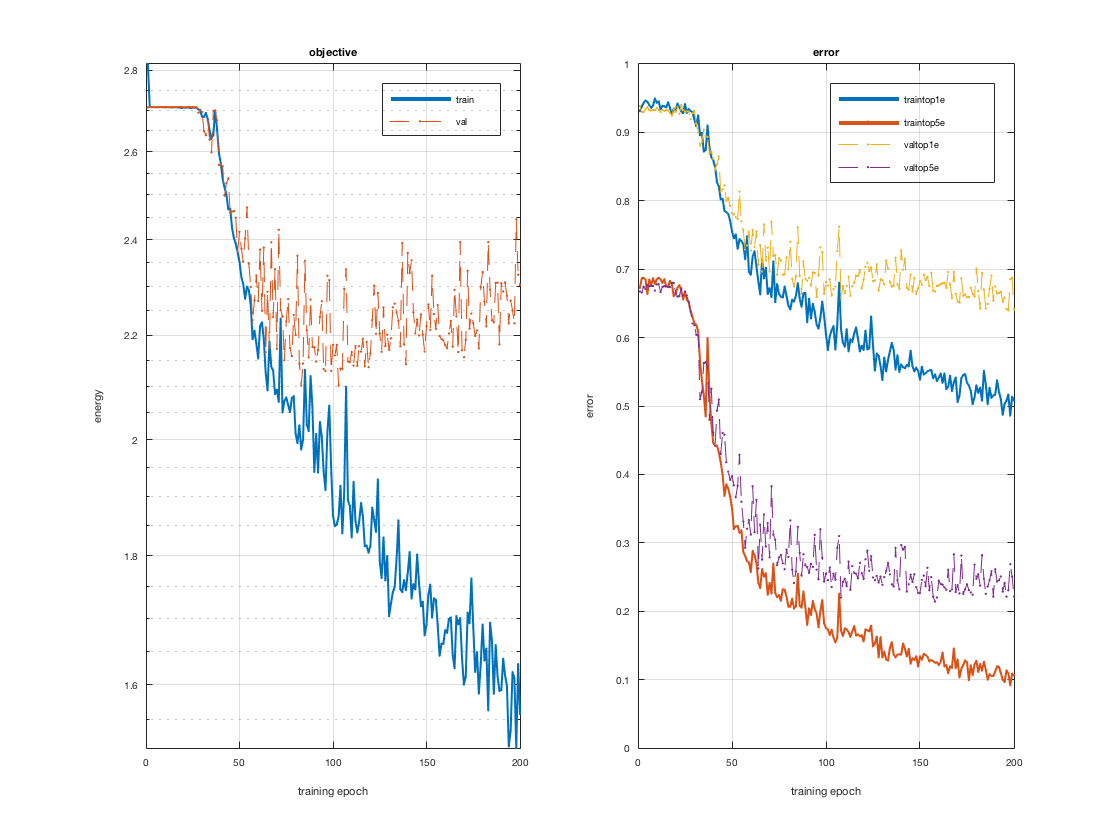
\includegraphics[width=0.9\textwidth]{Plots/3_50_200.png}
                \caption{using a Dropout of 50\%}
        \end{figure}
        followed by 25\% dropout resulting in 0.68 error 
        \begin{figure}[H]
            \centering
                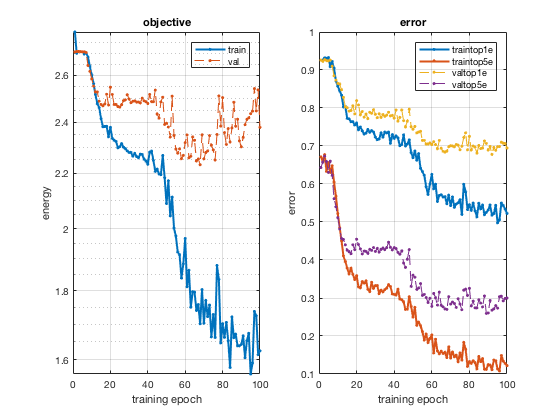
\includegraphics[width=0.9\textwidth]{Plots/3_25_200.png}
                \caption{using a Dropout of 25\%}
        \end{figure}
        and 75\% Dropout resulting in around 0.80 error.
        \begin{figure}[H]
            \centering
                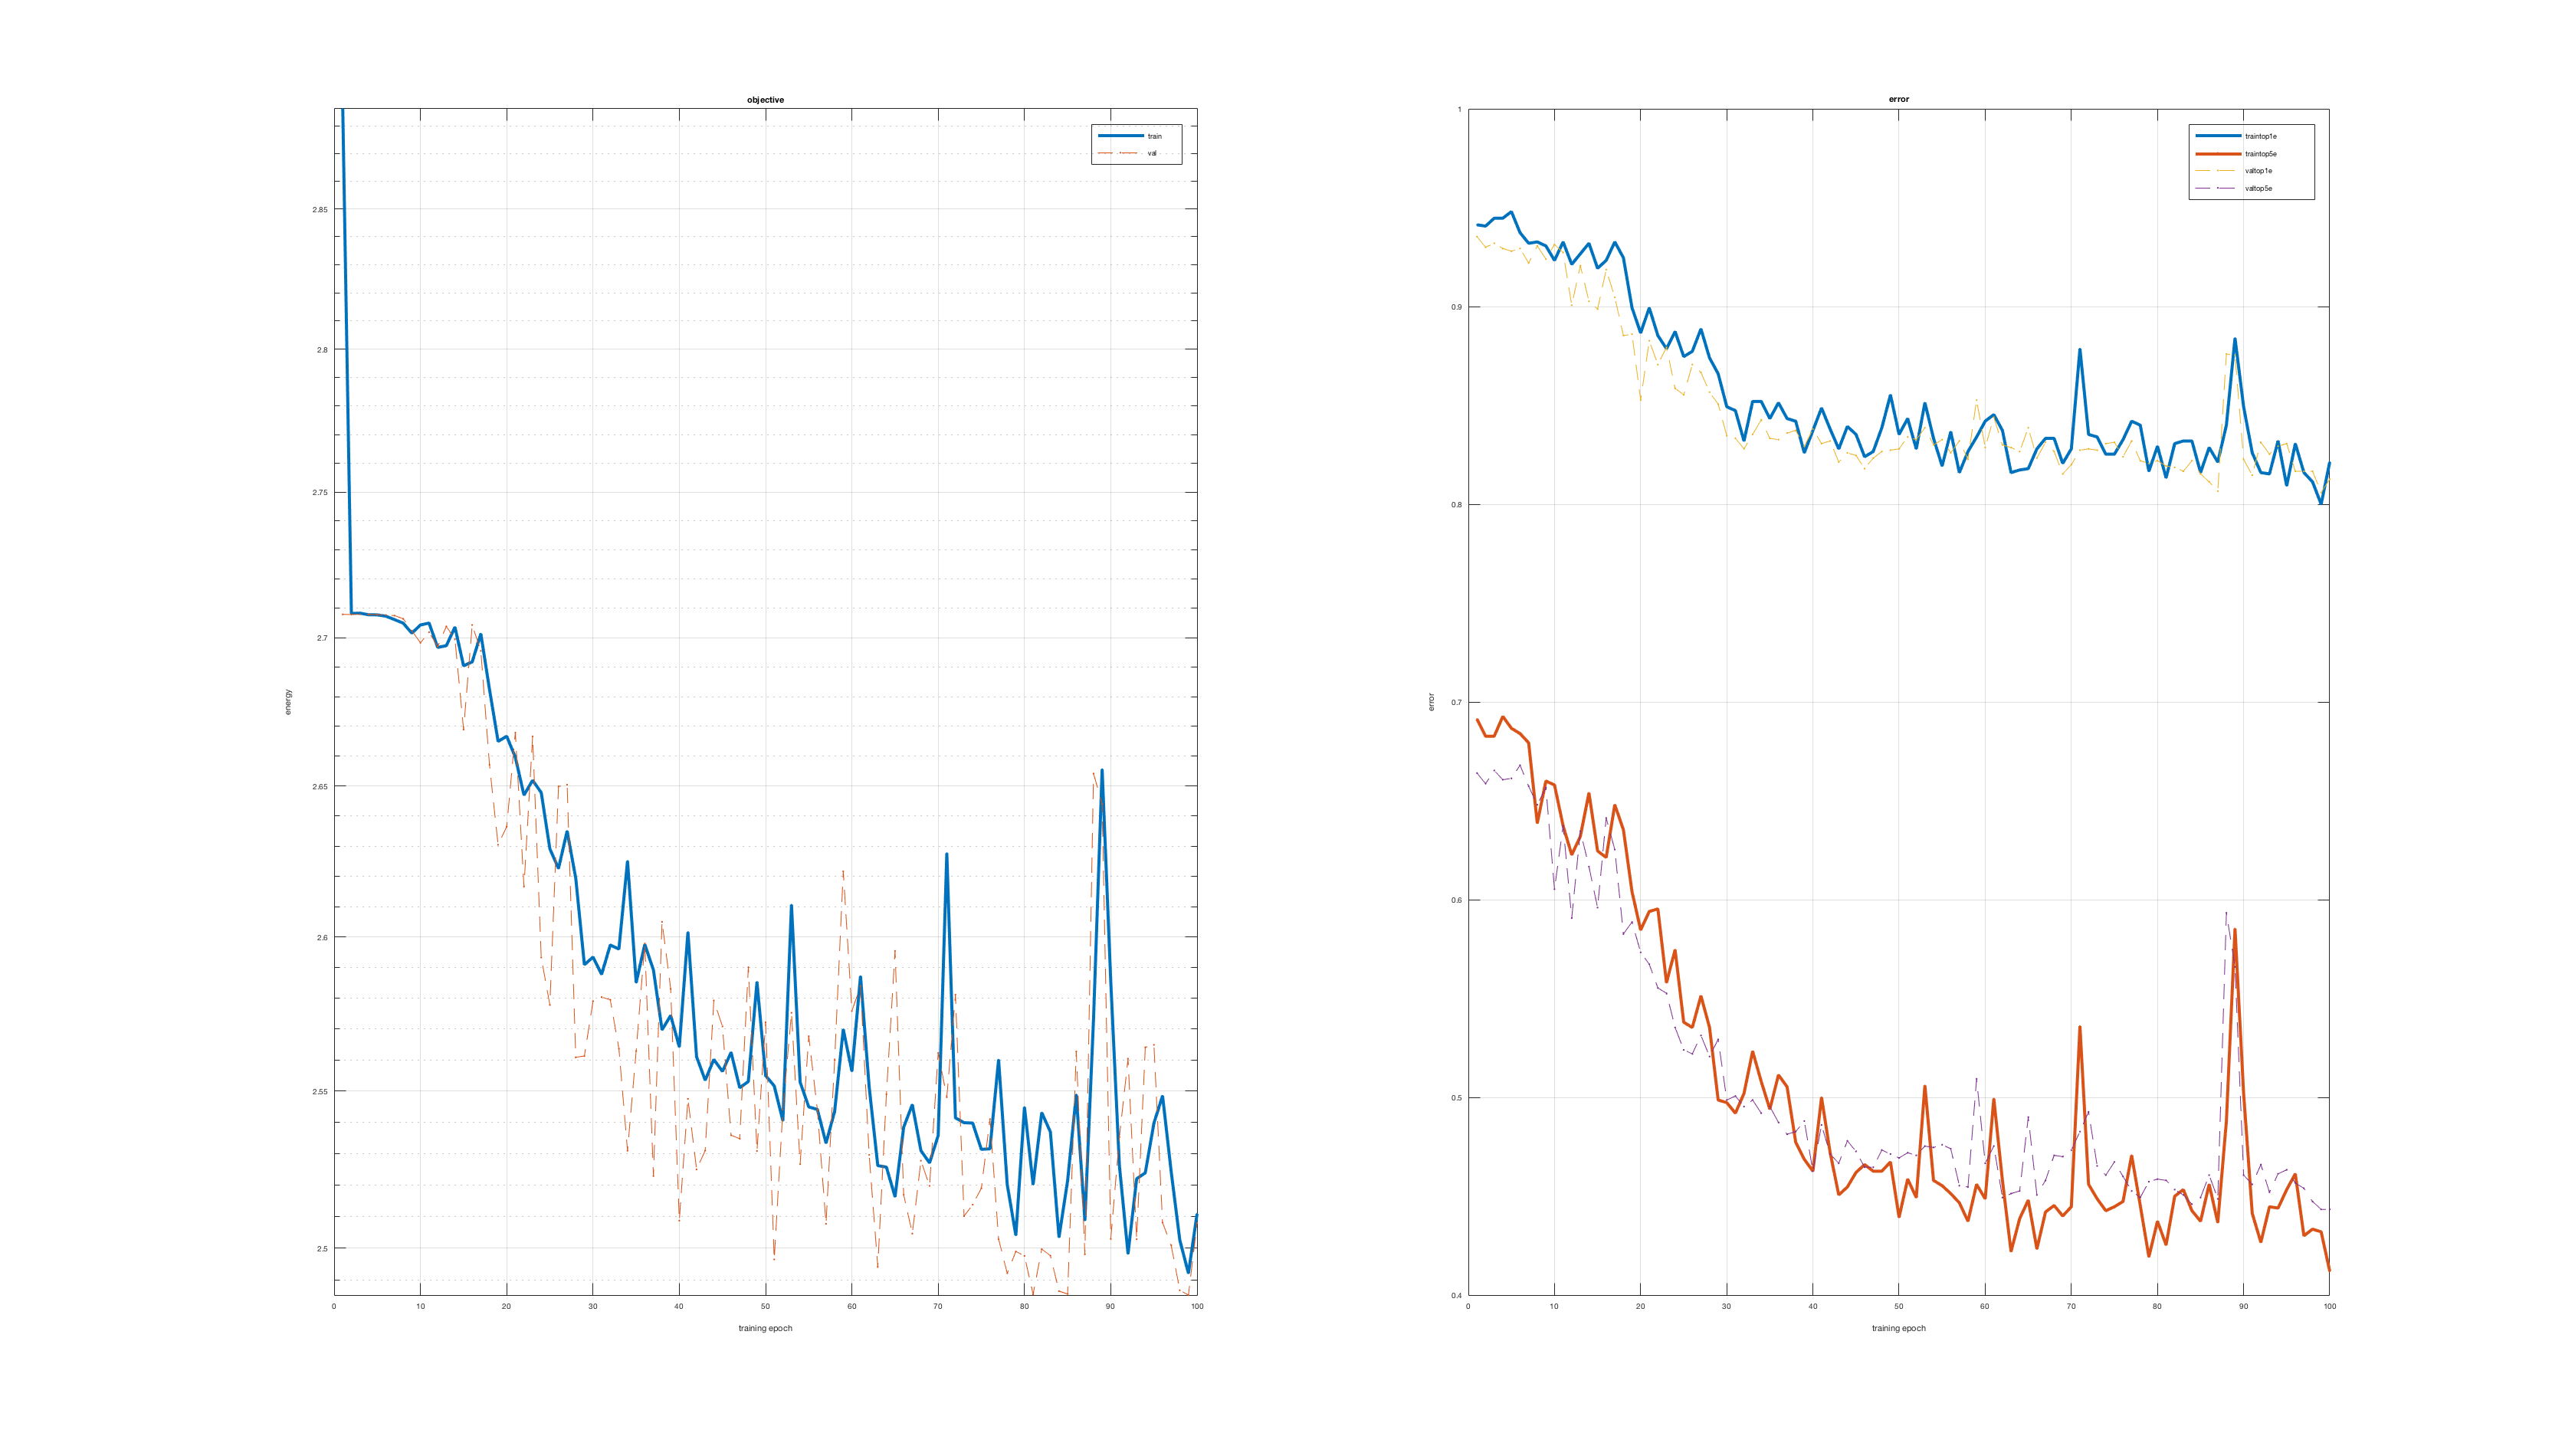
\includegraphics[width=0.9\textwidth]{Plots/3_75_100.png}
                \caption{using a Dropout of 75\%}
        \end{figure}
        Intuitively a dropout rate that is to high should result in a high test-error since the remaining network (after the dropout) is likely to weak to make meaningful predictions, which makes it difficult to learn from them. A dropout rate that is to low would allow more overfitting, which again leads to a higher test-error. Thus it makes sense that a dropout rate of 50\%, which lies in the middle of the other more extreme values, yields the best results.
\end{enumerate}


\newpage
\section{CNN with more Layers and Tricks}

        \begin{figure}[H]
            \centering
                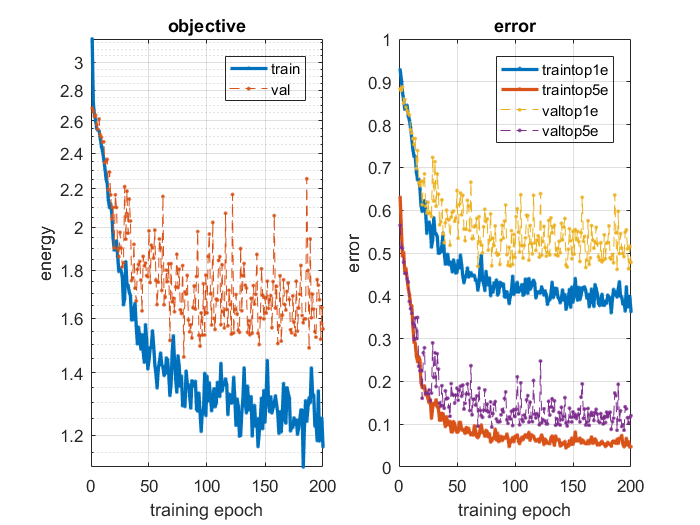
\includegraphics[width=0.9\textwidth]{Plots/q4_plot_epo_200.png}
                \caption{our Result using all the optimizations meantioned}
        \end{figure}
        We are achieving an error of only 0.48, which is a significant improvement to the 0.72 without any of the optimizations!
        \begin{figure}[H]
            \centering
                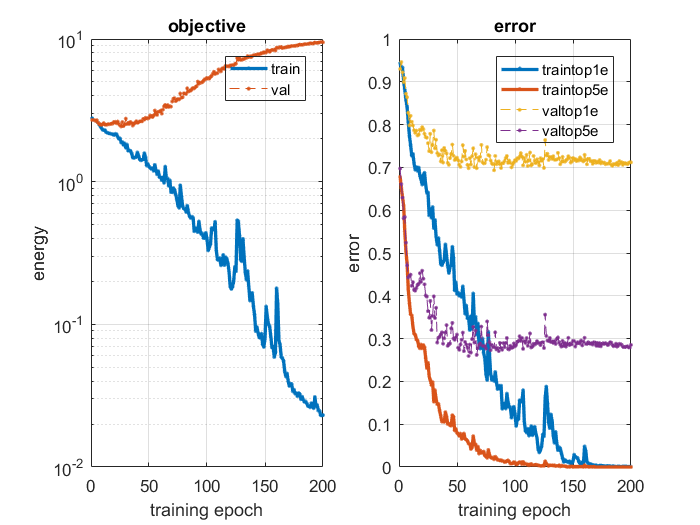
\includegraphics[width=0.9\textwidth]{Plots/init_plot_epo_200.png}
                \caption{our Result using no optimizations}
        \end{figure}

\section{Bonus}
We started implementing the bonus, but even if we change the input images to the correct resolution, subtract the mean and correct them to 3-channel images, the network will still throw errors while training, complaining about mismatches in dimensions.

\end{document}
